%!TEX root = paper.tex
% \subsection{Services}\label{Services}

% We now describe the various services that are provided in PETra.
% Earlier, we discussed the distributed ledger, which permanently
% stores valid transactions.  Below, we introduce the anonymous
% communication service, the mixing service for transaction anonymity,
% the anonymous bid storage, and smart-meter based billing.

\subsection{Communication Anonymity}
\label{comm} 
The anonymous communication layer is the infrastructure upon which all
other anonymity services in PETra are built.  The goal of communication anonymity is to allow smart meters and users to exchange transactions and bids without revealing their IP-addresses or other information which can be used to identify them. In almost all cases, at the very least the Internet Service Provider (ISP) has information about the users' communications and identities. The goal of this section is to maximize the anonymity to such an extent that not even ISPs can identify users. Existing protocols for low-latency communication anonymity include onion routing ~\cite{reed1998anonymous} or the similar garlic routing \cite{Liu2014EmpiricalMA}, STAC \cite{7986314} and the decentralized Matrix protocol.\footnote{Open-federated protocol for instant messaging, Voice-over-IP and IoT communications (\url{https://matrix.org/}).} In this section, we present a brief survey of onion and garlic routing, especially with respect to application in PETra.

% \begin{figure}
%  \centering
%  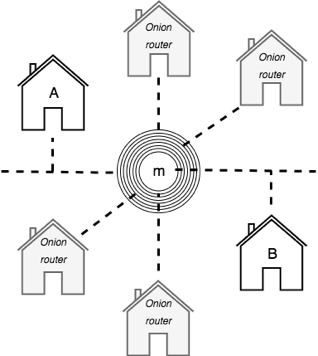
\includegraphics[width=0.6\columnwidth]{onionrouting.png}
%  \caption{Conceptual visualization of onion routing between smart meters to secure communication anonymity. In the figure, smart meter A is sending a message m, with final destination B, through the onion routers.}\label{fig:onionrouting}
%  \end{figure}
 
\subsubsection{Onion and Garlic Routing}
Onion routing is based on messages in communication being encapsulated in multiple layers of encryption and sent through a number of nodes in a network, called onion routers. It is anonymous because no single node, except for the sender and the receiver, can know the origin and the recipient of the message. In Figure \ref{fig:garlicrouting}, an example shows how smart meter A encrypts a message $m$, with final destination G, through a network of onion routers. A encrypts the message, for example a confirmation of an energy purchase, a certain number of times, along with addresses of members of the onion network. Each subsequent node, selected by the sender and specified in the different layers of encryption, decrypts one layer using its private key, revealing the next node to which the encrypted message is forwarded. Finally, the second to last node reveals the address of smart meter G and sends the still encrypted message to G, who can decrypt it safely. No single node in the network, except for the sender, knows how many times the packages is re-routed, and no node except for the sender and recipient can know their internal position in the chain of routing. Another technique for communication anonymity is called \textit{garlic routing}. It differs from onion routing in that multiple messages are encrypted together to counter tracing attacks.

\begin{figure}
\centering
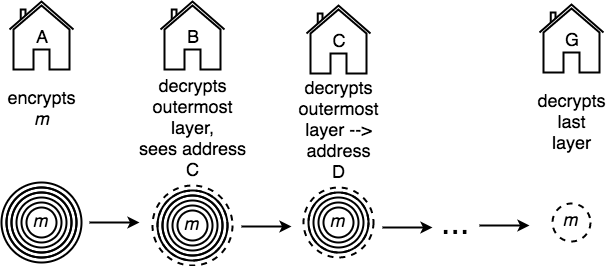
\includegraphics[width=\columnwidth]{garlicrouting.png}
\caption{The principle behind onion and garlic routing. The difference being that in onion routing, \textit{m} is a single message, whereas in garlic routing, \textit{m} is multiple messages packaged together.}\label{fig:garlicrouting}
\end{figure}

In practice, the deployment of onion routing (or a variant thereof called garlic routing) in the Invisible Internet Project (I2P) works as follows. Each node in the network operates an I2P router, allowing for anonymous communications. A router is distinct from an endpoint application in that it is not a secret who runs a router. By contrast, an application is the destination for the communications and is anonymous.  This disconnect allows for a higher degree of anonymity. To communicate between routers, unidirectional tunnels are set up. The tunnels use layered encryption, meaning that each router in the tunnel only can decrypt one layer. In order to transmit a message between two routers, the sender needs to know  where to direct the message, i.e., what the address of the entry point of the receiver is. 

The I2P protocol differs from regular network communications in that, for communications to take place between routers, each router needs to know a structure called the \textit{RouterInfo}. It contains the 2048-bit ELGamal encryption key, a signing key, a certificate, timestamp, text field, signature of bundle and the contact addresses where a router can be reached. The RouterInfo is given along with something called a \textit{LeaseSet}, containing a group of tunnel entry points for a particular client destination, when the tunnel will expire, the destination itself, encryption key for end-to-end encryption of garlic messages, revocation key and a signature of the LeaseSet data. The LeaseSet identifies an application on the I2P network. The I2P protocol ensures the anonymity of its users because of the disconnect between the identities of the applications communicating over the network, and the identities of the routers. This metadata is stored in a distributed directory called the netDb, based on the Kademlia P2P-protocol, which describes a provably consistent and fault-tolerant distributed hash table~\cite{kademlia}. The RouterInfo and LeaseSet data are stored on the netDb under the key derived from the SHA256 of the destination.


\subsubsection{Threat Vectors in Onion and Garlic Routing}
\label{commthreat} 
	Murdoch and Danezis \cite{1425067} show that a low-cost traffic analysis is possible of the Tor-network, theoretically and experimentally. Traffic analyses are based on tracking the forwarding of the size of a data package between computers, for example, if computer A sends a package of exactly 42 bytes to computer J, who then sends a package of exactly 42 bytes to B, it can be easily deduced that A sent a package of unknown content to computer B. This is possible because of the distribution of metadata to all routers in the Tor-network~\cite{Hopper:2010:MAN:1698750.1698753}. In what is called a timing analysis attack, an attacker tries to find a correlation between the timing of messages moving through the network to gain information about user identities and their communications. Analyses have shown that these types of attacks can be very effective over a wide range of network parameters when specific defences are not employed~\cite{Levine2004,4797313}.  To counter timing analysis attacks, the I2P network bundles multiple messages together (principle of garlic routing) and renders it more difficult to analyse~\cite{Liu2014EmpiricalMA}. Schimmer, 2009, showed that the bandwidth opportunistic peer-selection and -profiling algorithm does not prioritize anonymity in favor of performance~\cite{peerProfiling:2009}. Herrmann and Grothoff, 2011, exposed a potential weakness in anonymous HTTP-hosting done over the I2P network \cite{Herrmann2011}. The arguably only practical attack against the I2P network was done against the directory, the netDb, by Egger \textit{et al.} \cite{Egger2013}. An improvement of the protocol, aimed at Egger \textit{et al.}'s attack was suggested by Timpanaro \textit{et al.}, 2015 \cite{Timpanaro2015}. 
    
Another potential weakness of onion routing and garlic routing is that, even though the actual message is encrypted and the destinations are unknown, there is always a trace of the communication at the ISP level. The fact that a connection took place will be logged and is openly visible at the very least to the ISP. This attack can be countered in PETra by each node transacting and participating in the mixing network, regardless of the need for trading at that time. Trading of ``zero''-assets can help obfuscate the non-zero-assets of others. Another liability in onion and garlic routing can be that the legitimacy of the sender can not be immediately verified. This can be achieved by the techniques described in the section Transaction Anonymity.  


 
\subsubsection{Proposed Solution}
Given the survey of the previous paragraphs, performing P2P energy trading in transactive grids over a garlic routing network protocol such as the I2P network provides a high amount of communication anonymity for users. Only part of the energy trading in PETra will be anonymized by garlic routing, namely the internet connections. PETra is no different from other network communications in that aspect. The particularity of the trading being local and thus IP-addresses being close, is a potential weakness that can be countered by creating ``fake'' IP-addresses. To apply garlic routing to transactive microgrids, the smart meters, prosumers, and DSO can act as onion routers, and distribution of available routers is done over netDb. In practice, this service
can be built on the free and open-source I2P software
 with private
Directory Authorities.  In this case, anonymous communication
identifiers in bids and asks correspond to public-keys that identify
I2P applications.
% ritter.vg: "run your own tor network"
% https://ritter.vg/blog-run_your_own_tor_network.html


